\section{Segurança em redes}
\label{sec:seguranca}

A segurança no nível de rede indica uma área de pesquisa muito importante, já que os usuários estão continuamente colocando seus dados em ambientes em nuvem e mais dados são transferidos através de grandes distâncias. A razão para esta evolução é a crescente popularidade dos serviços em nuvem, bem como a simplicidade e rápida capacidade dos recursos sob demanda. Os impactos variam de acordo com os tipos de ameaças, e como defesa são criados diversos sistemas de segurança que agem como barreira de proteção, como por exemplo, \textit{firewalls}. Os principais tipos de ameaças são estudados a seguir. Também é apresentado um estudo mais detalhado do ataque do tipo varredura, foco deste trabalho.

\subsection{Tipos de ameaças}
Dos diversos tipos de ameaças que podem ocorrer nas redes de computadores, destacam-se algumas que são notórias por causar frequentes transtornos aos usuário, tais como:
\begin{itemize}
\item \textbf{Fraude} - Segundo Houaiss, Villar e Francisco \cite{Houaiss:2001}, é "qualquer ato ardiloso, enganoso, de má-fé, com intuito de lesar ou ludibriar outrem, ou de não cumprir determinado dever; logro". Esta categoria engloba as notificações de tentativas de fraudes, ou seja, de incidentes em que ocorre uma tentativa de obter vantagem, sejam por meios como correios eletrônicos não solicitados em massa (\textit{spam}) e páginas falsas.
    
\item \textbf{Ataque de negação de serviço (\textit{\gls{dos}}} - Um ataque de negação de serviço busca sobrecarregar serviços na rede dificultando o seu uso por usuários legítimos. Esse tipo de ataque, por sua natureza, pode produzir variações no volume de tráfego que normalmente são visíveis no gráfico de fluxo. Segundo Sperotto  \cite{Sperotto:2010} no entanto, na detecção de intrusão por fluxo, é abordado implicitamente o problema de ataques \gls{dos} por força bruta, ou seja, um tipo de \gls{dos} que depende de esgotamento de recursos ou sobrecarga da rede. Infelizmente, é quase impossível de detectar diretamente ataques \gls{dos} semânticas.
    
\item \textbf{Infestações viróticas automatizadas (\textit{Worms})} - São pequenos programas de computador criados para causar danos na máquina infectada e se auto replica pela rede, tirando cópias de si em cada computador \cite{Sperotto:2010}.
    
\item \textbf{Exército de máquinas controladas sem autorização (\textit{Botnets})} - Grupo de computadores comprometidos, chamados de computadores zumbis que são controlados remotamente por um centro de controle. \textit{Botnets} são muito utilizados para lançamento de ataques  como \textit{spams}, DoS e \textit{worms} \cite{Sperotto:2010}.
    
\item \textbf{Varredura de portas maliciosa (\textit{port scans})} - Técnica utilizada para encontrar fraquezas de um computador ou de uma rede. Enquanto esta técnica não é um ataque real, os hackers a usam para detectar quais portas estão abertas em um computador. Baseado nas informações sobre portas abertas, o acesso não autorizado pode ser obtido.
\end{itemize}

Os métodos citados também podem ser utilizados em conjunto, como por exemplo a utilização de \textit{botnets} que, controlados remotamente, podem efetuar ataques \gls{dos} a um mesmo servidor e ao mesmo tempo. A esse tipo de ataque é dado o nome de Negação de Serviço Distribuída (\gls{ddos})

Do ponto de vista de segurança, existe uma quantidade crescente de incidência de ataques de negação de serviço, \gls{dos}, durante os últimos anos \cite{Seeber:2015}. Além disso, segundo a \gls{cert.br}, responsável por tratar incidentes de segurança e computadores que envolvam redes conectadas à Internet brasileira, foram reportados 647.112 incidências de segurança somente no ano de 2016, sendo mais da metade (59\%), ataques do tipo \textit{port scan}.

\subsection{Técnicas de varredura}
\label{sec:varredura}

Um dos tipos mais comuns de ataques, a varredura consiste no envio de diversos tipos de pacotes com o intuito de se conhecer mais sobre o nó alvo ou a rede em questão. Através das respostas obtidas para esses pacotes, o atacante é capaz de chegar a diversas informações que possam ajudar em futuros ataques de diversos tipos. Alguns tipos de informações que podem ser descobertas incluem (não somente): A atividade dos servidores, informações relativas a softwares utilizados no sistema, informações sobre o \textit{firewall} e topologia da rede.

Uma das principais dificuldades nas soluções desse tipo de ataque é que as varreduras são consideradas atividades legais, e ocorrem na Internet de forma rotineira, inclusive com fins não maliciosos.

Antes de explorar as técnicas de varredura, faz-se necessário o entendimento de alguns conceitos de comunicação \gls{tcp}. Para obter um serviço \gls{tcp}, uma conexão necessita ser efetivada entre os computadores origem e destino. Esta conexão é realizada através dos chamados \textit{sockets}, formados pelo par endereço \gls{ip} e número de porta, de ambos, computador de origem e computador de destino. Entre estes dois \textit{sockets} ocorre a transferência de segmentos.

Um segmento consiste em um cabeçalho \gls{tcp} seguido, opcionalmente, por informação. Um cabeçalho \gls{tcp} pode possuir seis \textit{flags} que podem ser ativadas ou desativadas ao mesmo tempo \cite{Comer:1988}, são elas:

\begin{itemize}
    \item \textbf{SYN} - \textit{bit} de sincronismo, é o \textit{bit} que informa que este é um dos dois primeiros segmentos de estabelecimento da conexão.
    \item \textbf{ACK} - \textit{bit} de reconhecimento, indica que o valor do campo de reconhecimento está carregando um reconhecimento válido.
    \item \textbf{PSH} - \textit{bit} de \textit{push}, este mecanismo, que pode ser acionado pela aplicação, informa ao \gls{tcp} origem e destino que a aplicação solicita a transmissão rápida dos dados enviados, mesmo que ela contenha um número baixo de \textit{bytes}, não preenchendo o tamanho mínimo do \textit{buffer} de transmissão.
    \item \textbf{RST} - \textit{bit} de \textit{reset}, informa o destino que a conexão foi abortada neste sentido pela origem
    \item \textbf{FIN} - \textit{bit} de terminação, indica que este pacote é um dos pacotes de finalização da conexão.
\end{itemize}

Em uma comunicação \gls{tcp}, uma conexão deve ser estabelecida entre os dois pontos (\textit{sockets}) para que a transferência de dados ocorra.
Inicialmente a máquina emissora, também chamada de cliente, transmite um segmento cuja \textit{flag} SYN é de 1 (para assinalar que se trata de um segmento de sincronização), com um número de ordem X, que se chama número de ordem inicial do cliente.

A seguir, a máquina receptora, chamada de servidor, recebe o segmento inicial que provém do cliente e envia-lhe um aviso de recepção, isto é, um segmento cuja \textit{flag} ACK é de 1 e a \textit{flag} SYN é de 1 (porque ainda se trata de uma sincronização). Este segmento contém o número de ordem do servidor, que é o número de ordem inicial do cliente. O campo mais importante deste segmento é o campo de aviso de recepção, que contém o número de ordem inicial do cliente, incrementado de 1.

Por último, o cliente transmite ao servidor um aviso de recepção, ou seja, um segmento cuja \textit{flag} ACK é de 1, cuja \textit{flag} SYN é de zero (não se trata mais de um segmento de sincronização). O seu número de ordem é incrementado e o número de aviso de recepção representa o número de ordem inicial do servidor, incrementado de 1.

Depois dessa sequência de trocas (Figura \ref{fig:troca-tcp}), também chamada de \textit{handshake}, ou, aperto de mãos em português, as duas máquinas estão conectadas e a comunicação pode ser efetivada.

\begin{figure}[H]
  \centering
  \caption{Estabelecimento de conexão TCP}
  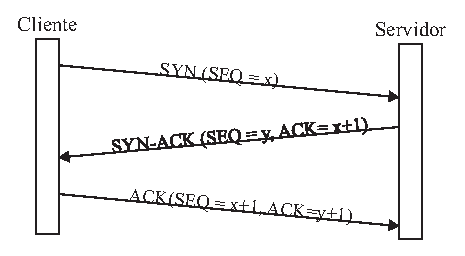
\includegraphics[width=0.5\textwidth]{images/conexao-tcp.eps}
  \label{fig:troca-tcp}
   \fonte{Elaborado pelo autor.}
\end{figure}
\FloatBarrier

Os passos a seguir são definidos pela RFC 793 \cite{rfc793}, utilizada pela grande maioria das implementações \gls{tcp} e exploradas em técnicas de varredura.

\begin{itemize}
    \item Quando um segmento SYN chega em um aporta aberta, é continuado o procedimento de \textit{handshake} como discutido anteriormente; 
    \item Quando um segmento SYN (ou FIN) chega em uma porta fechada, o segmento é descartado e um segmento RST é retornado para o cliente;
    \item Quanto um segmento FIN chega em uma porta que esteja aberta, o segmento é descartado.
    \item Quando um segmento RST chega em uma porta que esteja ouvindo (aberta), o segmento é descartado;
    \item Quando um segmento RST chega em uma porta que não esteja ouvindo (fechada), o segmento é descartado;
    \item Quando um segmento ACK chega à uma porta aberta, o mesmo é descartado e retornado um segmento RST.
\end{itemize}


Devido à sua natureza, \textit{scans} podem facilmente criar um vasto número diferente de fluxos.
Há três categorias de \textit{scans}: \textit{scan} horizontal - onde um \textit{host} varre uma porta especifica em diferentes \textit{hosts}; \textit{scan} vertical - um \textit{host} verifica várias portas em um outro \textit{host} específico; e \textit{block scan} que é a combinação dos dois \cite{Sperotto:2010}.

Existem várias técnicas de varredura de porta disponíveis e podem facilmente ser automatizadas por ferramentas como Nmap \cite{Lyon:2009}. Alguns métodos utilizados para varredura serão estudados a seguir \cite{deVivo:1999, Christopher:2001}.

\textbf{\textit{TCP Connect}} - É a forma mais comum de \textit{scanning}. Basicamente uma conexão TCP regular (\textit{handshake} completo) para cada porta definida na varredura. Para cada porta, a conexão pode resultar em sucesso, indicando uma porta aberta ou em falha caso contrário. Essa técnica é facilmente implementada pois não necessita de privilégios especiais e, do mesmo modo, é facilmente detectável. Através de \textit{logs} do sistema alvo é possível verificar mensagens de requisição de conexão e de erro para as conexões negadas. Neste método, o \textit{scanner} envia uma mensagem SYN para o sistema alvo. Se uma porta estiver (aberta) ouvindo com um serviço, a conexão se sucederá. Um SYN é retornado estabelecendo o número de sequência inicial. Um ACK considera o campo numérico de confirmação válido. Se a porta estiver (fechada) sem serviço ouvindo, uma mensagem RST é retornada, para reiniciar o pedido de conexão. Alguns exemplos de \textit{scanners} podem ser Nmap, Amap e Blaster. %Exemplo de \textit{scanner}: nmap.

\textbf{TCP SYN} - Também conhecida por \textit{Half Open} por não explorar um \textit{handshake} completo. Nesta técnica o \textit{scanner} envia uma mensagem SYN, como se estivesse pedindo uma conexão. Se responder como um RST, indica que a porta está fechada, e uma nova porta é testada. Se a resposta da máquina alvo for um SYN/ACK, indica que a porta se encontra ouvindo. O \textit{scanner} envia então um RST cancelando o \textit{handshake}. A vantagem desse tipo de \textit{scanning} é o fato de, mesmo ainda podendo ser detectado, tentativas de conexões SYN são menos frequentemente registradas se comparadas com conexões \gls{tcp} completas. %Exemplos de \textit{scanners}: amap, hping2, netstat, nmap.

\textbf{Exploração FIN} - Neste método, quando um segmento FIN é enviado para uma porta fechada, o computador alvo responde com um TCP RST. Quando a porta estiver aberta, o segmento é ignorado e o computador alvo não responde. O \textit{scanner} não recebe nunhuma resposta, pois não podem pertencer a uma conexão estabelecida. %Exemplos de \textit{scanners}: hping2, nmap.

\textbf{Xmas Tree} - é uma variação do método TCP FIN, neste, são utilizadas mensagens com prioridade TCP FIN/URG/PSH. Quando estiver ouvindo, o \textit{host} alvo não responde, caso contrário, responde com um TCP RST. %Exemplos de \textit{scanners}: hping2, netstat, nmap.

\textbf{TCP Null (sem flags ativos)} - também é uma variação do método TCP FIN, neste, tem-se resposta para portas fechadas, mas não para portas abertas.% Exemplos de \textit{scanners}: hping2, netstat, nmap.

\textbf{Varredura ACK} - Técnica utilizada para identificar \textit{firewalls}. Um segmento ACK que não pertença a nenhum conexão é gerado pelo \textit{scanner}. Se um RST é devolvido pela máquina alvo, tanto em uma porta aberta como em uma fechada, as portas são classificadas como não tendo \textit{firewall}.

\textbf{Varredura ARP} - Não se trata exatamente de varredura de portas mas essa técnica é utilizada para descobrir dispositivos ativos na rede local, para depois realizar a varredura de portas somente nos computadores ativos. O \textit{scanner} envia uma série de pacotes de protocolo \gls{arp} \cite{RFC0826} e incrementa o valor do \gls{ip} alvo a cada \textit{broadcast}.



\subsection{Ferramentas de Varredura}

Para que as varreduras sejam efetuadas, tem-se a possibilidade de utilizar ferramentas que possibilite a varredura utilizando as diferentes formas citadas na seção anterior. Uma das ferramentas mais utilizadas, e que foi utilizada neste trabalho é o Nmap \cite{Lyon:2009}.

O Nmap é um \textit{software} que oferece uma gama muito grande de recursos e funcionalidades, como detecção do Sistema Operacional remoto, o serviço e a versão que está em uso no host, o exame de ociosidade por identificação (ID) de Internet Protocol (IP), o rápido exame de multiportas por ping entre tantas outras. Possui versões para plataformas Unix, Windows, e MacOS sendo utilizado tanto por interface console como também em interface gráfica. O software Nmap é um utilitário livre e de código aberto, usado para exploração de redes, segurança e auditoria, capaz de examinar grandes redes ou simplesmente um único host.
A função principal do Nmap é realizar uma varredura em portas \gls{tcp} e o retorno dessa varredura é classificado em um dos seguintes estados: aberta, fechada, filtrada, não filtrada e a combinação de aberta/filtrada ou fechada/filtrada \cite{Lyon:2009}. Vários outros softwares que são utilizados para gerencia e controle de redes de computadores fazem uso do Nmap pois pode ser usado diretamente, sempre que se desejar uma verificação de portas em um \textit{host} que esteja em uma rede local ou na Internet.
O uso mais simples do Nmap é escanear diretamente uma máquina da rede, onde uma quantidade enorme de portas \gls{tcp} será examinada na máquina alvo, e cada porta será classificada de acordo com seu estado.
Na linha de comando do Nmap, tudo que não for uma opção ou argumento de opção será tratado como uma especificação de hospedeiro alvo. O caso mais simples é a especificação de um endereço IP ou nome de hospedeiro alvo para exame \cite{Lyon:2009}.


\subsection{Sistemas de detecção e prevenção de intrusão}

O isolamento da rede em redes virtuais permite uma maior segurança devido ao seu isolamento, porém problemas tradicionais relacionados à segurança continuam existindo em ambientes virtualizados pois 60\% a 70\% dos ataques à segurança da rede são de origem interna segundo Lynch (2006) \nocite{Lynch:2006}. Uma das formas de se proteger desses ataques é monitorar o tráfego em busca de atividades maliciosas ou violação de políticas. Para realizar o monitoramento de pacotes na rede, a solução mais apropriada é o sistema de detecção de intrusão, que realiza o monitoramento passivo dos pacotes na rede. Porém, esse tipo de análise não permite que sejam tomadas ações para prevenir tais ataques, e então faz se necessário um sistema de prevenção de intrusão para bloquear esses pacotes.

Segundo Kruegel (2014) \nocite{Kruegel:2004}, "Detecção de intrusão é o processo de identificar e responder à atividades maliciosas na computação e redes de dados". Uma tentativa de intrusão, também chamada de ataque, refere-se a uma série de ações em que um intruso tenta obter o ganho do sistema. O objetivo de um \gls{ids} é discriminar tentativas de intrusão e preparação de intrusão do uso normal do sistema.

Infelizmente, arquiteturas \gls{ids}/\gls{ips} utilizadas atualmente possuem muitas barreiras para gerir nós distribuídos. Em redes tradicionais, para detectar e prevenir intrusos maliciosos na rede de dados, administradores normalmente necessitam implantar diversos detectores de intrusão em diferentes locais da rede, e então analisar dados do tráfego coletados localmente ou em um nodo centralizado. Como as configurações dependem da topologia da rede, configurações manuais e mudanças frequentes são inevitáveis para tornar a política em nós distribuídos eficaz e coerente. Além disso, algoritmos de detecção de intrusão eficazes normalmente são desenhados para um determinado tipo de ataque. Para desenvolver sistemas de detecção eficazes, mais e mais protocolos de proteção são criados, o que resulta na redução do desempenho da rede. Além disso, dispositivos de rede normalmente possuem protocolos proprietários, o que torna mais difícil desenvolver interfaces de gerenciamento automáticas \cite{Wang:2015}.

Vários trabalhos para \gls{ids} tem sido desenvolvidos desde o início de sua pesquisa nos anos 1980. Essas propostas podem ser classificadas de acordo com várias características, como tipo de dados analisado (\textit{logs} ou dados do pacote), tipo de análise (em tempo real ou \textit{offline}) ou pelo tipo de processamento (centralizado ou distribuído). No entanto, os modelos de classificação mais conhecidos são os baseados em assinatura e os baseados em anomalia \cite{Kolpyakwar:2017}.

Sistemas de detecção de intrusão baseados em assinatura realizam a detecção através da comparação de dados do pacote com uma base de dados conhecida. O \gls{ids} Snort \cite{Roesch:1999} é um dos exemplos mais utilizados dessa técnica, verificando padrões de pacote através da análise de dados da carga útil (\textit{payload}) do pacote. O Snortik \cite{Fagundes16} também é um bom exemplo, neste, é proposto uma integração entre o \gls{ids} Snort e o sistema de \textit{firewall} do sistema MikroTik RouteOS \cite{mikrotik16} com a finalidade de automatizar o processo de reação à ataques. \glspl{ids} baseados em assinatura possuem alta precisão, raramente apresentando alarmes para fluxos normais, porém, não reconhecem fluxos novos, não presentes na sua base de dados. Além disso, a inspeção de pacotes é difícil e até mesmo impossível de ser realizada  em redes com taxas com múltiplos Gigabits por segundo \cite{Lai:2004, Gao:2006}.

Sistemas de detecção de intrusão baseados em anomalia por sua vez, comparam dados recebidos com um "modelo de normalidade" que descreve o comportamento normal da rede. Alterações significativas desse modelo são consideradas como anomalias. Exemplos de criação de comportamentos podem ser redes neurais, técnicas de análise de estatísticas e teoria das probabilidades. A principal vantagem desse tipo de detecção é o fato de também detectar fluxos não conhecidos anteriormente \cite{Owezarski:2010}. No entanto, podem existir casos em que fluxos podem ser diferentes da normalidade esperada mas não necessariamente serem maliciosos resultando em alarmes falsos positivos.

Um \gls{ids} deve ser capaz de lidar com o número crescente do tráfego e ataques na rede. No entanto, alternativas baseadas nas análise de carga útil possuem eficácia em redes entre 100Mbps e 200Mbps \cite{Lai:2004, Gao:2006} podendo chegar a 1Gbps quando hardware dedicado é empregado \cite{Vasiliadis:2008}. Sistemas como Bro \cite{Paxson:1999} e Snort \cite{Roesch:1999} apresentam alto consumo de recursos  quando confrontado com a enorme quantidade de dados de alta taxa de transferência encontrados \cite{Dreger:2004}. Além disso, protocolos criptografados podem representar um desafio a mais para sistemas de carga útil. Para redes de alta taxas de transmissão, alternativas à inspeção de pacotes são muito importantes. Uma dessas alternativas e que tem atraído pesquisadores é a detecção de intrusão de anomalias baseada em fluxo.

Com esta abordagem, são analisados os padrões de comunicação dentro da rede, ao invés do conteúdo dos pacotes individuais. Hoje em dia os sistemas de medição especiais são capazes de fornecer, para cada par de endereços IP e números de porta, informações agregadas, como a quantidade de bytes transferidos, o número de pacotes enviados e o tempo que determinado fluxo de dados esteve ativo. Essas informações podem então ser exportadas para outros sistemas analisarem, para então, serem usados para detectar intrusões \cite{Sperotto:2010}.

Considerando essa inflexibilidade sobre os equipamentos atuais, os interesses sobre abstrair funções de rede de \textit{switches} dedicados para aplicações \gls{sdn} vem aumentando. Sendo assim, as políticas de segurança podem ser instaladas pelo controlador como regras nas tabelas de fluxo \cite{Kim:2013}, em vez de configurações manuais e independentes. Com isso, o \textit{switch} provê apenas a função de filtro de acordo com a regra na tabela de fluxo, não influenciando significativamente no desempenho da rede. Além disso, \gls{sdn} tem recursos naturais de estatísticas que são úteis para a análise de detecção de intrusão, de modo que o controlador obtém mais visibilidade sobre o tráfego da rede. Portanto, \gls{sdn} parece fornecer uma arquitetura mais adequada para \gls{ips}.